% A vote-counting path for the ballot problem with a = 5, b = 3:
% each up-step is a vote for Alice, each down-step a vote for Bob,
% and the path stays strictly above zero after the first step.
% Fills upstream's \missingfigure{path} in
% book/tex/measure/martingale.tex (§ The ballot problem).
\documentclass[border=2mm]{standalone}
\usepackage{tikz}
\begin{document}
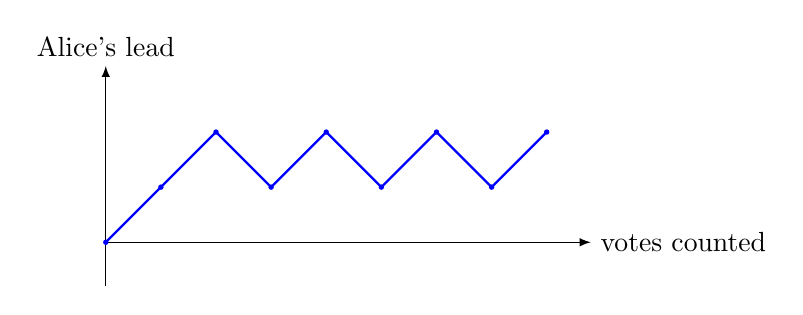
\begin{tikzpicture}[scale=0.7,>=latex]
  % Axes.
  \draw[->] (0,0) -- (8.8,0) node[right] {votes counted};
  \draw[->] (0,-0.8) -- (0,3.2) node[above] {Alice's lead};
  % The path: A A B A B A B A (a = 5, b = 3).
  \draw[thick, blue]
    (0,0) -- (1,1) -- (2,2) -- (3,1) -- (4,2) -- (5,1)
          -- (6,2) -- (7,1) -- (8,2);
  \foreach \x/\y in {0/0,1/1,2/2,3/1,4/2,5/1,6/2,7/1,8/2}
    \fill[blue] (\x,\y) circle (1.4pt);
\end{tikzpicture}
\end{document}
